% CVPR 2026 Paper Template; see https://github.com/cvpr-org/author-kit

\documentclass[10pt,twocolumn,letterpaper]{article}
 
%%%%%%%%% PAPER TYPE  - PLEASE UPDATE FOR FINAL VERSION
% \usepackage{cvpr}              % To produce the CAMERA-READY version
\usepackage[pagenumbers]{cvpr}
\usepackage{float}
\usepackage{placeins}
% \usepackage[pagenumbers]{cvpr} % To force page numbers, e.g. for an arXiv version

% Import additional packages in the preamble file, before hyperref
\input{preamble}

% It is strongly recommended to use hyperref, especially for the review version.
% hyperref with option pagebackref eases the reviewers' job.
% Please disable hyperref *only* if you encounter grave issues, 
% e.g. with the file validation for the camera-ready version.
%
% If you comment hyperref and then uncomment it, you should delete *.aux before re-running LaTeX.
% (Or just hit 'q' on the first LaTeX run, let it finish, and you should be clear).
\definecolor{cvprblue}{rgb}{0.21,0.49,0.74}
\usepackage[pagebackref,breaklinks,colorlinks,allcolors=cvprblue]{hyperref}

%%%%%%%%% PAPER ID  - PLEASE UPDATE
\def\paperID{*****} % *** Enter the Paper ID here
\def\confName{CVPR}
\def\confYear{2026}

%%%%%%%%% TITLE - PLEASE UPDATE
\title{Explainable Multi-Stage Deep Learning for \\ 
Brain Tumor Segmentation and Classification}

%%%%%%%%% AUTHORS - PLEASE UPDATE
\author{Bow Wing Yin\\
{\tt wybow@connect.ust.hk}
\and
Lai Yui Chun \\
{\tt yclaiaj@connect.ust.hk}
\and
Chan Ho Yan \\
{\tt hychandr@connect.ust.hk}
}

\raggedbottom  

\begin{document}
\maketitle
\begin{abstract}
Brain tumors exhibit substantial morphological and malignancy variability, leading to misdiagnosis rates exceeding 20\% with routine MRI 
interpretation and delaying neuro-oncology interventions. We propose an explainable, multi-stage deep learning framework that integrates
 tumor segmentation, classification, and structured summary generation to create a clinical decision support system. The pipeline first employs 
 a ResUNet to localize tumor regions on MRI slices. It then uses predicted masks to extract region-of-interest (ROI) crops, combines them 
 with the original full image in a dual-input architecture, and feeds the result to a fine-tuned ResNet50 classifier to predict one of four 
 classes: glioma, meningioma, pituitary tumor, or no tumor. The system provides explainability through Grad-CAM heatmaps and a MedGemma VLM that generates structured clinical summaries with a deterministic template fallback for reliability.
  Moreover, the quantitative stage-consistency metrics and qualitative 
  evaluations confirm strong alignment across pipeline stages. We used extensive ablation studies and qualitative evaluations to demonstrate
   that the framework delivers high performance while producing clinically coherent, trustworthy explanations.

\end{abstract}   
\section{Introduction}

Brain tumors exhibit substantial variability in morphology, anatomical location, and malignancy, making accurate MRI-based diagnosis challenging. Conventional radiological assessment can suffer from high misdiagnosis rates because tumor appearance varies across patients and tumor types~\cite{yan2016mri}. Recent deep learning methods have shown strong performance for brain tumor classification and segmentation, but many models remain difficult to interpret. This limits their usefulness in clinical decision support, where clinicians need not only a prediction but also evidence showing where the model is looking and whether the decision is consistent with visible tumor regions.

We propose an explainable multi-stage deep learning framework for brain tumor MRI analysis. The pipeline first uses ResUNet to segment the tumor region, then uses the predicted mask to extract an ROI crop. To reduce information loss from cropping, the final classifier uses a dual-input ResNet50 design that combines the ROI crop with the original full MRI image. The system further provides visual explanations using Grad-CAM and generates structured clinical summaries using a MedGemma-based VLM with a deterministic fallback template. This design aims to balance predictive performance with interpretability by linking the final classification decision to explicit localization, visual attention, and textual explanation.

Using the Kaggle Brain Tumor MRI Dataset and the SciDB mask-annotated dataset, our experiments show that ResUNet achieves the best segmentation overlap among the evaluated segmentation backbones, reaching a Dice score of 0.7431 and IoU of 0.6558. For classification, the dual-input ResNet50 achieves 99.00\% accuracy and 98.95\% F1-score, approaching the full-image baseline while preserving the localization benefits of segmentation-guided classification. Ablation experiments show that increasing the ROI margin improves cropped-only classification, but the dual-input design is more effective because it restores global anatomical context. VLM comparisons further show that MedGemma provides the best task-specific summary quality among the evaluated summary-generation models.

\section{Related Work}

\subsection{Architectural Paradigms in Tumor Segmentation 
}For medical image segmentation, recent research shows a difference between generalized foundation models and specialized convolutional architectures. The effectiveness of an Attention-Enhanced U-Net is demonstrated by recent studies which use attention gates to suppress unimportant background features and concentrate on intricate tumor structures \cite{Islam2026}. Conversely, the SAMed-2 framework \cite{Yan2025} explores the adaptation of the "Segment Anything" architecture into a medical foundation model, leveraging temporal adapters and memory mechanisms for zero-shot generalization across datasets. Our proposed pipeline makes use of a ResUNet architecture, as opposed to the high computational requirements of foundation models like SAMed-2. This method maintains multi-scale spatial details and guarantees stable gradient flow by incorporating residual blocks into the U-Net structure. This choice validates that for specialized medical applications, a residual-based encoder-decoder provides a highly pragmatic compute-accuracy trade-off without the extensive pretraining or hardware requirements of foundation models. 

\subsection{Enhancing Classification through Localization and Transfer Learning }
Although there are many different approaches to feature extraction, deep transfer learning is still a fundamental component of tumor classification. The usefulness of applying pre-trained networks, such as Xception and DenseNet, directly on complete MRI slices is highlighted \cite{Asif2022}, which optimizes hyperparameters to attain high accuracy on benchmarks. Similar to this, an improved classification framework based on a Deep Multiple Fusion Network (DMFN) is also proposed \cite{Vure2025}. This method reduces inter-class overlap by breaking down the multi-class classification problem into a number of pairwise binary classifications using ResNet18. Rather than using complex ensemble fusions or processing the entire MRI scan, our proposed system takes a segmentation-guided multi-stage approach. The pipeline explicitly crops out irrelevant anatomical context by converting the predicted segmentation mask into a localized ROI before passing the image to a fine-tuned ResNet50 classifier. While full-image models may occasionally capture peripheral cues, this explicit localization requires the classifier to base its decision solely on the targeted tumor region. 

\subsection{Explainability, Reliability, and Summary Generation}
The transition from predictive accuracy to clinical trustworthiness depends heavily on explainable AI and reliable summary-generation mechanisms. Islam et al.~\cite{Islam2026} use Gradient-weighted Class Activation Mapping (Grad-CAM) to generate heatmaps that highlight spatial features contributing to a classification label. This method is useful for checking whether a network focuses on tumor pathology or irrelevant background structures. However, incorporating these maps into a multi-stage workflow remains challenging. Our proposed system addresses this by computing the intersection-over-union (IoU) between the segmentation mask and the Grad-CAM activation as a quantitative stage-consistency metric. This checks whether the localization and classification stages attend to the same pathology and adds an objective layer of verification to qualitative heatmaps.

Beyond visual evidence, the rise of VLMs in medical summary generation has introduced concerns about hallucinations and unconstrained generative output. The CALM-VLM framework~\cite{Dhinagar2026} addresses this issue through selective prediction: by applying temperature scaling to the model's probability distributions, it estimates uncertainty and abstains from producing a summary when prediction entropy is too high. Our proposed pipeline investigates a structural reliability alternative. Instead of relying only on statistical abstention, our VLM produces structured summaries with findings, impressions, and recommendations, while a deterministic class-conditioned fallback is used when the generated text is malformed or inconsistent with the classifier prediction. This keeps the textual explanation grounded in the verified visual prediction.

 
 
\section{Data}
\label{sec:data}
The data used in this project consists of 2D brain MRI slices for a multi-class brain tumor classification and segmentation task. 
It comprises grayscale (single-channel) medical imaging data, where each sample is a 2D slice labeled as one of four categories—glioma, 
meningioma, pituitary tumor, or no tumor. The primary source is the publicly available Brain Tumor MRI Dataset hosted on Kaggle, containing 
approximately 7,200 human brain MRI images distributed across the four classes, supplemented by the SciDB Brain Tumor Dataset, which provides
 the T1-weighted contrast-enhanced images. We did not collect new data, and the project relies entirely on these two publicly available sources.

 The dataset was divided into stratified train/validation/test splits (80/10/10) to preserve class distribution and mitigate imbalance. For segmentation, the mask-annotated data are split into 1753 training images, 219 validation images, and 220 test images. For classification, the stratified split contains 5618 training images, 702 validation images, and 703 test images.

We addressed class imbalance through weighted cross-entropy loss based on inverse class frequency for classification, and a combined BCE--Dice loss for segmentation to handle the severe foreground-background disparity typical of tumor regions. During training, we apply online data augmentation: random spatial and intensity transformations with joint image-mask processing for segmentation, and random rotation, horizontal flipping, and brightness/contrast jittering for classification. No additional heavy filtering was required. Preprocessing mainly consists of consistent resizing, mask alignment, and online augmentation, all implemented in PyTorch.
    
\section{Methods}
\label{sec:methods}
Our system follows a modular multi-stage design: an input MRI slice is first segmented to localize the tumor region, the predicted tumor region is cropped and resized, and a classifier predicts one of four classes: glioma, meningioma, pituitary tumor, or no tumor. Finally, Grad-CAM and a summary-generation module are used to provide visual and textual explanations for the prediction.



\subsection{Tumor Localization with ResUNet}
For tumor localization, we use a ResUNet-based~\cite{zhang2018resunet} binary segmentation model. Given an MRI slice $I$, the network predicts a soft tumor mask $\hat{M} \in [0,1]^{H \times W}$, where higher values indicate tumor likelihood. At inference time, a threshold of 0.5 is applied to obtain the final binary mask.

We choose the U-Net~\cite{ronneberger2015unet} family because it is well suited to medical image segmentation with limited annotated data. Its encoder-decoder structure captures semantic context, while skip connections preserve spatial details needed for tumor boundaries. Compared with classification-only CNNs, U-Net directly optimizes pixel-level localization. We also considered more automated or foundation-model-based alternatives such as nnU-Net~\cite{isensee2021nnunet} and SAM-style promptable models~\cite{kirillov2023segment}, but a 2D U-Net-family model offered a better compute-accuracy trade-off for our project timeline.

Our final segmentation model is ResUNet, a residual variant of U-Net. ResUNet keeps the same encoder-decoder and skip-connection structure, but replaces plain convolutional blocks with residual blocks. This improves gradient flow and optimization stability, especially when the network becomes deeper. Since brain tumor regions can vary strongly in size, contrast, and boundary shape, the residual design helps preserve useful low-level and high-level features during mask prediction.

We also evaluated standard U-Net and Attention U-Net as alternatives. Standard U-Net serves as the simplest encoder-decoder baseline, while Attention U-Net tests whether attention gates on skip connections can suppress irrelevant background features. 
Based on the segmentation comparison in Table~\ref{tab:seg-results}, ResUNet performs the best overall, so it is used as the final tumor localization model in the proposed pipeline.
Figure~\ref{fig:segmentation_example} shows an example MRI slice and its corresponding predicted tumor mask produced by the ResUNet segmentation model.


\begin{figure}[!htbp]
    \centering
    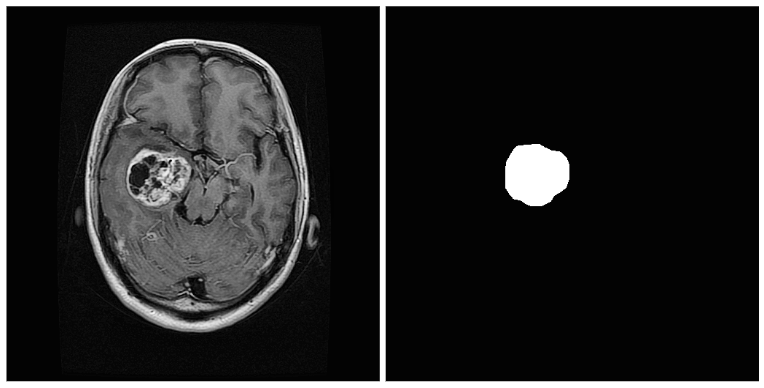
\includegraphics[width=0.5\linewidth]{figures/mri_segmentation_example.png}
    \caption{Left: original brain MRI slice. Right: predicted binary segmentation mask highlighting the tumor region.}
    \label{fig:segmentation_example}
\end{figure}

\subsection{Segmentation Objective}
The segmentation models are trained using a combination of BCE loss and Dice loss. BCE treats segmentation as an independent binary classification problem at each pixel:
\begin{equation}
    \mathcal{L}_{BCE}
    =
    -\frac{1}{N}
    \sum_{i=1}^{N}
    \left[
    M_i \log(\hat{M}_i)
    +
    (1-M_i)\log(1-\hat{M}_i)
    \right],
\end{equation}
where $N$ is the number of pixels, $M_i \in \{0,1\}$ is the ground-truth label for pixel $i$, and $\hat{M}_i \in [0,1]$ is the predicted tumor probability. BCE encourages pixel-wise correctness and provides stable gradients during optimization.

However, tumor segmentation is highly class-imbalanced because the tumor usually occupies only a small portion of the MRI slice. In this setting, a model can achieve low BCE by predicting mostly background. To address this, we also use Dice loss, which directly measures foreground overlap between the predicted mask and the ground-truth mask. The Dice similarity coefficient is defined as:
\begin{equation}
    DSC(\hat{M}, M)
    =
    \frac{2|\hat{M} \cap M| + \epsilon}
    {|\hat{M}| + |M| + \epsilon},
\end{equation}
where $\epsilon$ is a small smoothing constant for numerical stability. Dice loss is then:
\begin{equation}
    \mathcal{L}_{Dice}
    =
    1 - DSC(\hat{M}, M).
\end{equation}
 
The final segmentation objective is:
\begin{equation}
    \mathcal{L}_{seg}
    =
    \lambda \mathcal{L}_{BCE}
    +
    (1-\lambda)\mathcal{L}_{Dice},
\end{equation}
where $\lambda=0.5$ in our experiments. This combined objective balances pixel-level accuracy from BCE with region-level overlap from Dice loss. Such Dice-based objectives are widely used in medical image segmentation because they are more robust to foreground-background imbalance than pixel accuracy alone~\cite{milletari2016vnet,sudre2017generalised}. U-Net-style medical segmentation methods also commonly rely on overlap-based losses or metrics to evaluate tumor-region quality~\cite{ronneberger2015unet}.



\subsection{Segmentation-Guided Classification}
For the segmentation-guided setting, the predicted mask, illustrated in Figure~\ref{fig:segmentation_example}, is converted into a ROI proposal for classification.

We first apply connected-component analysis to the binary mask and select the largest connected component as the predicted tumor region. A bounding box is then fitted around this component and expanded by a 20-pixel margin to preserve nearby anatomical context. The corresponding region is cropped from the original MRI slice and resized to the standard ResNet50 input resolution before classification. If no ROI is available, such as for no-tumor images or empty predicted masks, the full image is resized and used instead. We use this fixed input size because ResNet50 is initialized with ImageNet-pretrained weights, making the fine-tuning setup consistent with the pretrained model while controlling computational cost.

For the final classification setting, we use a dual-input design that combines the segmentation-guided ROI crop with the original full MRI image. The ROI crop provides localized tumor-focused information, while the full image preserves global anatomical context that may be lost during cropping. This design allows the classifier to remain tied to the segmented tumor region while reducing the information loss observed in cropped-only classification.
Figure~\ref{fig:roi_cropping} illustrates this ROI cropping process, where the predicted tumor mask is used to localize the lesion and extract a tumor-centered patch for classification.

\begin{figure}[!htbp]
    \centering
    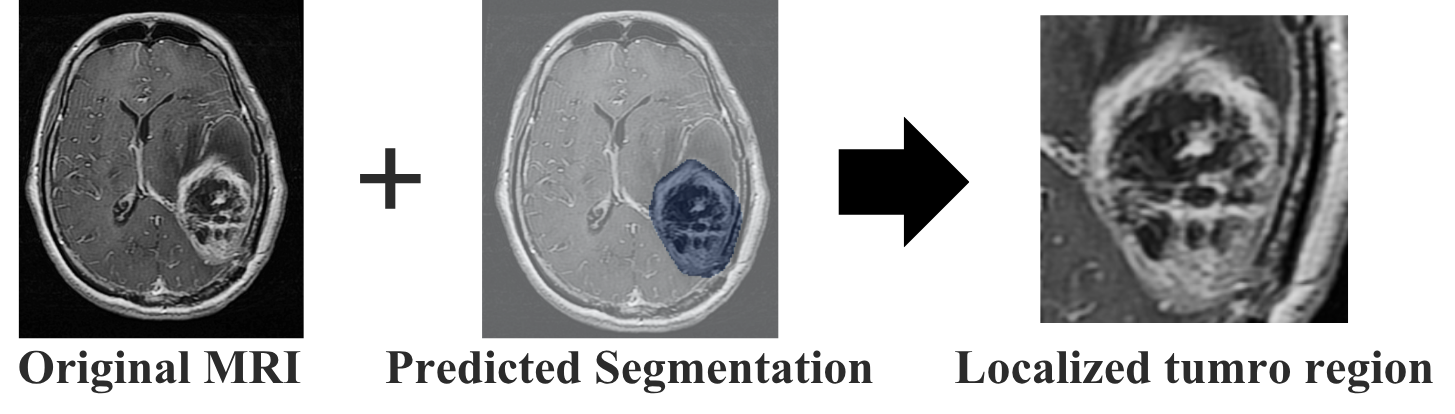
\includegraphics[width=0.97\linewidth]{figures/roi_cropping_example.png}
    \caption{Segmentation-guided ROI cropping for classification.}
    \label{fig:roi_cropping}
\end{figure}

The classifier is based on ResNet50 pretrained on ImageNet~\cite{he2016resnet}. We choose ResNet50 because its residual connections support deep feature learning while reducing vanishing-gradient issues, making it suitable for distinguishing visually similar tumor categories. Compared with larger modern architectures such as Vision Transformers, which typically require larger datasets or more extensive pretraining~\cite{dosovitskiy2021vit}, ResNet50 is a practical transfer-learning backbone for our moderate-sized medical dataset, where fine-tuning pretrained CNNs has been shown to be effective~\cite{tajbakhsh2016convolutional}.

We replace the final fully connected layer with a task-specific four-way classification layer and fine-tune the network using cross-entropy loss. To account for class imbalance, the loss is weighted by inverse class frequency:
\begin{equation}
    \mathcal{L}_{cls}
    =
    - \sum_{c=1}^{C} w_c y_c \log p_c ,
\end{equation}
where $C=4$, $w_c$ is the class weight, $y_c$ is the ground-truth label, and $p_c$ is the predicted probability.




\subsection{Explainability and Summary Generation}
To make the classification decision more interpretable, we use Grad-CAM to identify which image regions contribute most strongly to the ResNet50 prediction. Grad-CAM is applied to the final convolutional block of ResNet50, corresponding to \texttt{layer4} in our implementation. Given a predicted class $c$, Grad-CAM computes the gradient of the class score with respect to the feature maps in this layer. These gradients are then used to weight the feature maps, producing a coarse localization heatmap that highlights the regions most responsible for the prediction. As illustrated in Figure~\ref{fig:gradcam_process}, we normalize this heatmap and overlay it on the input MRI slice, allowing the classifier's attention to be visually compared with the tumor region predicted by the segmentation model.

\begin{figure}[H]
    \centering
    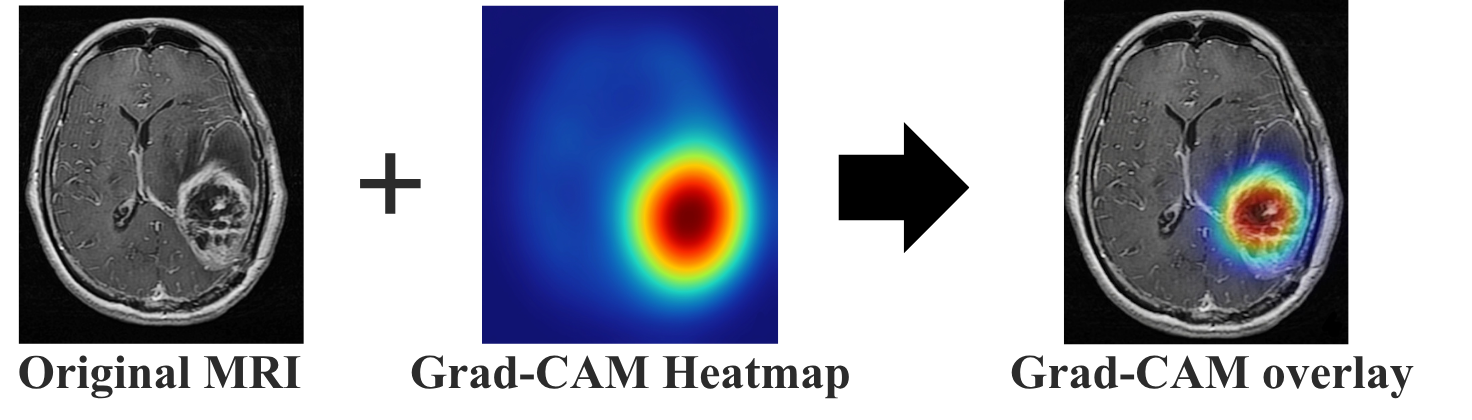
\includegraphics[width=\linewidth]{figures/gradcam_process.png}
    \caption{Grad-CAM visualization process. The heatmap is overlaid on the original MRI slice to highlight regions that contribute most strongly to the classifier prediction.}
    \label{fig:gradcam_process}
\end{figure}

This visual explanation also allows us to check whether the two stages of the pipeline are consistent with each other. To quantify this relationship, we compute a stage-consistency measure between the predicted segmentation mask and the Grad-CAM activation. The segmentation mask is binarized, and the Grad-CAM heatmap is thresholded to identify high-activation regions. We then measure their overlap using IoU. A high overlap suggests that the classifier is focusing on the tumor region proposed by the segmentation model, while a low overlap indicates that the classifier may be relying on background structures or other spurious image cues.

In addition to visual explanations, we generate a structured textual explanation for each prediction. The summary-generation module takes the predicted tumor class, model confidence, Grad-CAM focus region, and optionally the segmentation mask as inputs. It first attempts to produce a summary using a VLM-based generation step conditioned on this model evidence. We use a zero-shot instruction prompt that asks the model to generate three fixed sections: findings, impression, and recommendation. This prompt design is chosen because it does not require task-specific summary examples, while the fixed section format keeps the output clinically structured and easier to validate. If the generated output is unavailable, malformed, or inconsistent with the predicted class, the system falls back to a deterministic class-conditioned template. This hybrid VLM-template design keeps the summary aligned with the classifier output while still allowing more natural clinical language when generation succeeds.

\subsection{Training Strategy}
All models are optimized with Adam and early stopping. The segmentation models are trained using the combined BCE--Dice objective, while the ResNet50 classifier is trained using weighted cross-entropy. Training-time data augmentation is applied online to improve robustness, with random spatial and intensity transformations for segmentation, random rotation, horizontal flipping, and brightness/contrast jittering for classification. Exact hyperparameters are reported in Section~\ref{sec:experiments}.
\section{Experiments}
\label{sec:experiments}

\subsection{Experimental Setup}
All experiments use the train/validation/test splits for segmentation and classification described in Section~\ref{sec:data}.

For evaluation, segmentation performance is measured using Dice coefficient, IoU, and the 95th percentile Hausdorff distance (HD95). Dice and IoU measure overlap between the predicted and ground-truth tumor masks. HD95 measures boundary distance by reporting the 95th percentile of surface-to-surface distances, making it less sensitive to extreme outlier pixels than the standard Hausdorff distance. Classification performance is measured using accuracy, precision, recall, and F1-score.

The hyperparameters in Table~\ref{tab:optimization_details} were selected using validation performance and computational constraints. For classification, the learning rate and batch size were selected using a lightweight grid search over learning rates $\{10^{-3}, 5 \times 10^{-4}, 10^{-4}, 5 \times 10^{-5}\}$ and batch sizes $\{16, 32, 64\}$, with validation F1 as the selection criterion. The remaining settings follow the training configuration used in the pipeline.

\begin{table}[H]
    \centering
    \small
    \caption{Training hyperparameters used in the main experiments.}
    \label{tab:optimization_details}
    \setlength{\tabcolsep}{3pt}
    \makebox[\linewidth][c]{%
    \begin{tabular}{lcc}
    \hline
    Hyperparameter & Segmentation & Classification \\
    \hline
    Input size & $256 \times 256$ & $224 \times 224$ \\
    Optimizer & Adam & Adam \\
    Learning rate & $3 \times 10^{-4}$ & $5 \times 10^{-5}$ \\
    Weight decay & $1 \times 10^{-5}$ & $1 \times 10^{-4}$ \\
    Batch size & 8 & 32 \\
    Maximum epochs & 130 & 50 \\
    Early-stopping patience & 12 epochs & 10 epochs \\
    Scheduler & ReduceLROnPlateau & ReduceLROnPlateau \\
    Selection metric & Validation Dice & Validation F1 \\
    \hline
    \end{tabular}%
    }
\end{table}

Early-stopping patience denotes the number of consecutive epochs without validation-loss improvement before training is stopped.




\subsection{Segmentation Comparison}
To select the segmentation backbone, we compare U-Net, ResUNet, and Attention U-Net under the same data split, training protocol, and evaluation metrics. Table~\ref{tab:seg-results} shows that ResUNet achieves the best Dice and IoU, while U-Net obtains the lowest HD95. Since Dice and IoU better reflect overall tumor-region overlap, we select ResUNet as the final localization backbone.

\begin{table}[H]
\centering
\caption{Segmentation results on the test set.}
\label{tab:seg-results}
\begin{tabular}{lccc}
\hline
Model & Dice $\uparrow$ & IoU $\uparrow$ & HD95 $\downarrow$ \\
\hline
U-Net & 0.7102 & 0.6230 & \textbf{11.55} \\
ResUNet & \textbf{0.7431} & \textbf{0.6558} & 11.85 \\
Attention U-Net & 0.7360 & 0.6472 & 14.56 \\
\hline
\end{tabular}
\end{table}

Qualitative inspection suggests that the models usually identify the main tumor region, but common failure cases include small tumors, low-contrast boundaries, and irregular lesions where part of the tumor is missed.




\subsection{Classification Ablation}
We evaluate several classification settings to understand the effect of segmentation-guided cropping. The full-image ResNet50 baseline removes segmentation guidance and classifies the original MRI image directly. The cropped multi-stage variants use the predicted tumor ROI, with different bounding-box margins, to test whether the crop size limits classification performance. Finally, the dual-input model combines both the cropped ROI and the original full image, allowing the classifier to use localized tumor information while retaining global anatomical context.

\begin{table}[H]
    \centering
    \small
    \caption{Classification ablation results on the test set.}
    \label{tab:cls-results}
    \setlength{\tabcolsep}{1pt}
    \makebox[\linewidth][c]{%
    \begin{tabular}{lcccc}
    \hline
    Input setting & Accuracy & Precision & Recall & F1 \\
    \hline
    Full-image ResNet50 baseline & \textbf{0.9915} & \textbf{0.9914} & \textbf{0.9909} & \textbf{0.9911} \\
    Cropped ROI, 10-pixel margin & 0.9516 & 0.9498 & 0.9502 & 0.9496 \\
    Cropped ROI, 15-pixel margin & 0.9579 & 0.9476 & 0.9532 & 0.9504 \\
    Cropped ROI, 20-pixel margin & 0.9621 & 0.9520 & 0.9674 & 0.9596 \\
    Dual input: cropped ROI + full image & 0.9900 & 0.9895 & 0.9895 & 0.9895 \\
    \hline
    \end{tabular}%
    }
    \end{table}

Table~\ref{tab:cls-results} shows that increasing the ROI margin improves the cropped-only classifier, with the 20-pixel margin giving the best cropped result. However, the improvement from 10 to 20 pixels is modest compared with the remaining gap between cropped-only classification and the full-image baseline. Supplementary Figures~\ref{fig:supp_cm_resunet_single} and~\ref{fig:supp_cm_resunet_dual} show that the cropped-only model makes more cross-class mistakes among tumor categories, while the dual-input model reduces these errors by restoring global image context. This suggests that the main limitation is not only the crop margin, but also the loss of global anatomical context and the propagation of segmentation errors into the classifier input.

The dual-input model substantially reduces this gap by combining the localized tumor crop with the original full image. Its test F1-score reaches 0.9895, much closer to the full-image baseline than any cropped-only variant. The training curves in Supplementary Figures~\ref{fig:supp_dual_training_curves} and~\ref{fig:supp_dual_metric_curves} show stable optimization, with validation metrics converging to a high level. Although the full-image baseline still achieves the highest numerical performance, we use the dual-input setting for the final explainable pipeline because it preserves the interpretability benefits of segmentation-guided localization while recovering most of the global context needed for accurate classification.





\subsection{VLM Summary Generation Comparison}
We compare four VLMs for the summary-generation component: BLIP-2, InstructBLIP, CLIP, and MedGemma. The exact model checkpoints are listed in Table~\ref{tab:vlm-results}. The generated summaries are evaluated using reference-based text-similarity metrics and task-specific summary-quality metrics.

ROUGE-L measures the longest common subsequence overlap between the generated summary and the reference summary, capturing similarity in wording and sentence structure. METEOR measures word-level alignment while also considering more flexible matches such as stemming and synonyms. The keyword-hit rate measures whether clinically relevant tumor terms appear in the generated summary. The composite score summarizes task-specific summary quality by combining keyword coverage, confidence reporting, and length appropriateness.

\begin{table}[H]
    \centering
    \small
    \caption{VLM summary-generation comparison.}
    \label{tab:vlm-results}
    \setlength{\tabcolsep}{2pt}
    \makebox[\linewidth][c]{%
    \begin{tabular}{lcccc}
    \hline
    Model & ROUGE-L & METEOR & Keyword hit & Composite \\
    \hline
    blip2-opt-2.7b & 0.1526 & 0.1264 & 0.4909 & 0.7425 \\
    instructblip-vicuna-7b & 0.2408 & 0.2023 & 0.4491 & 0.6991 \\
    clip-vit-base-patch32 & \textbf{0.2716} & 0.2358 & 0.4109 & 0.7025 \\
    medgemma-1.5-4b-it & 0.1694 & \textbf{0.3431} & \textbf{0.6600} & \textbf{0.8300} \\
    \hline
\end{tabular}%
}
    \end{table}

Table~\ref{tab:vlm-results} shows that \texttt{clip-vit-base-patch32} achieves the highest ROUGE-L score, indicating the strongest longest-subsequence overlap with the reference summaries. However, \texttt{medgemma-1.5-4b-it} achieves the best METEOR score, keyword-hit rate, and composite score. This suggests that MedGemma produces summaries with better clinically relevant terminology and stronger task-specific alignment, even if its surface-level wording is less similar to the reference summaries. Therefore, we use medgemma-1.5-4b-it as the summary-generation model in the final pipeline.





\subsection{Explainability Analysis}
Grad-CAM visualizations are used to inspect whether the classifier focuses on clinically meaningful regions. In successful examples, the heatmap overlaps with the predicted segmentation mask, suggesting that the segmentation and classification stages rely on similar tumor evidence. In failure cases, the heatmap may activate outside the predicted tumor area or on high-contrast background structures, indicating possible reliance on spurious cues.

These visual checks complement the quantitative ablations by showing not only whether the model is correct, but also where its evidence comes from. This is important for the final pipeline because the prediction, localized ROI, Grad-CAM attention, and generated summary should be consistent with one another.
Supplementary Figures~\ref{fig:supp_debug_notumor}, \ref{fig:supp_debug_pituitary}, \ref{fig:supp_real_notumor}, \ref{fig:supp_real_pituitary}, and~\ref{fig:supp_real_glioma} show qualitative examples from the final pipeline, including the original MRI, segmentation output, Grad-CAM visualization, and generated summary.





\section{Conclusion}
We have developed a complete, modular, and explainable multi-stage deep learning pipeline for brain tumor segmentation and classification from 2D MRI slices. The ResUNet segmentation backbone achieves localization performance (Dice 0.7431, IoU 0.6558) and effectively focuses downstream classification while enabling robust interpretability. 

The dual-input ResNet50 classifier combines segmentation-guided ROI crops with full-image context and attains 99.00\% accuracy and 98.95\% F1-score. This helps address the accuracy-interpretability trade-off by recovering global anatomical context lost in pure ROI cropping, while still preserving explicit tumor localization.

Grad-CAM visualizations and a quantitative stage-consistency IoU metric verify that the classifier focuses on the same tumor regions identified by segmentation, providing an objective safeguard against spurious correlations. For textual explanations, MedGemma outperforms other VLMs (BLIP-2, InstructBLIP, CLIP) in clinically relevant terminology and composite summary quality; the hybrid MedGemma VLM + template approach reduces the risk of prediction-inconsistent summaries and keeps textual explanations aligned with model predictions.

\paragraph{Limitations and Future Work.}
Several limitations remain. First, the current pipeline processes 2D MRI slices independently and does not model volumetric context across adjacent slices. Future work could extend the segmentation stage to 3D U-Net or transformer-based architectures, which may improve localization of small or irregular tumors. Second, the VLM summary module still relies on a fallback template when generation is malformed or inconsistent with the classifier prediction. Incorporating calibrated uncertainty estimation or selective prediction could help the system decide when to generate free text and when to fall back to a safer template.

Third, our evaluation is based on publicly available datasets with relatively high-quality annotations, so additional validation on external datasets and other tumor types is needed to assess generalizability. The same multi-stage explainable framework could also be adapted to other medical imaging tasks, such as lung nodule assessment, diabetic retinopathy grading, or histopathology analysis. Finally, Grad-CAM and the segmentation-consistency metric provide useful evidence, but they do not guarantee clinical correctness. Future user studies with radiologists are needed to evaluate whether the combined visual and textual explanations improve diagnostic trust and decision making. Reducing computational overhead through model distillation or a shared backbone would also make the system more practical for deployment.

{
    \small
    \bibliographystyle{unsrtnat}
    \bibliography{main}
}
\clearpage
\onecolumn
\section*{Supplementary Material}

\subsection*{A. Additional Classification Ablation Figures}

\begin{figure}[H]
    \centering
    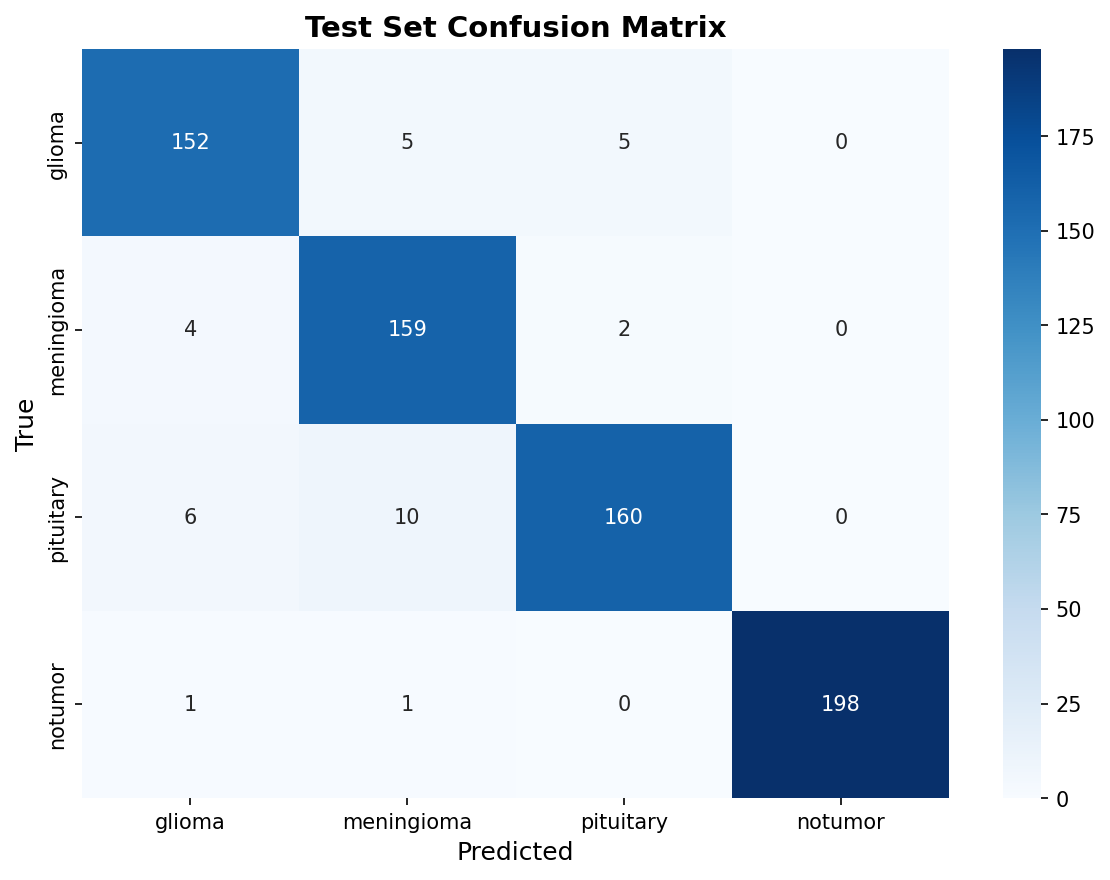
\includegraphics[width=0.5\textwidth]{figures/confusion_matrix_resunet_single.png}
    \caption{Confusion matrix for the cropped-only ResNet50 classifier.}
    \label{fig:supp_cm_resunet_single}
\end{figure}

\begin{figure}[H]
    \centering
    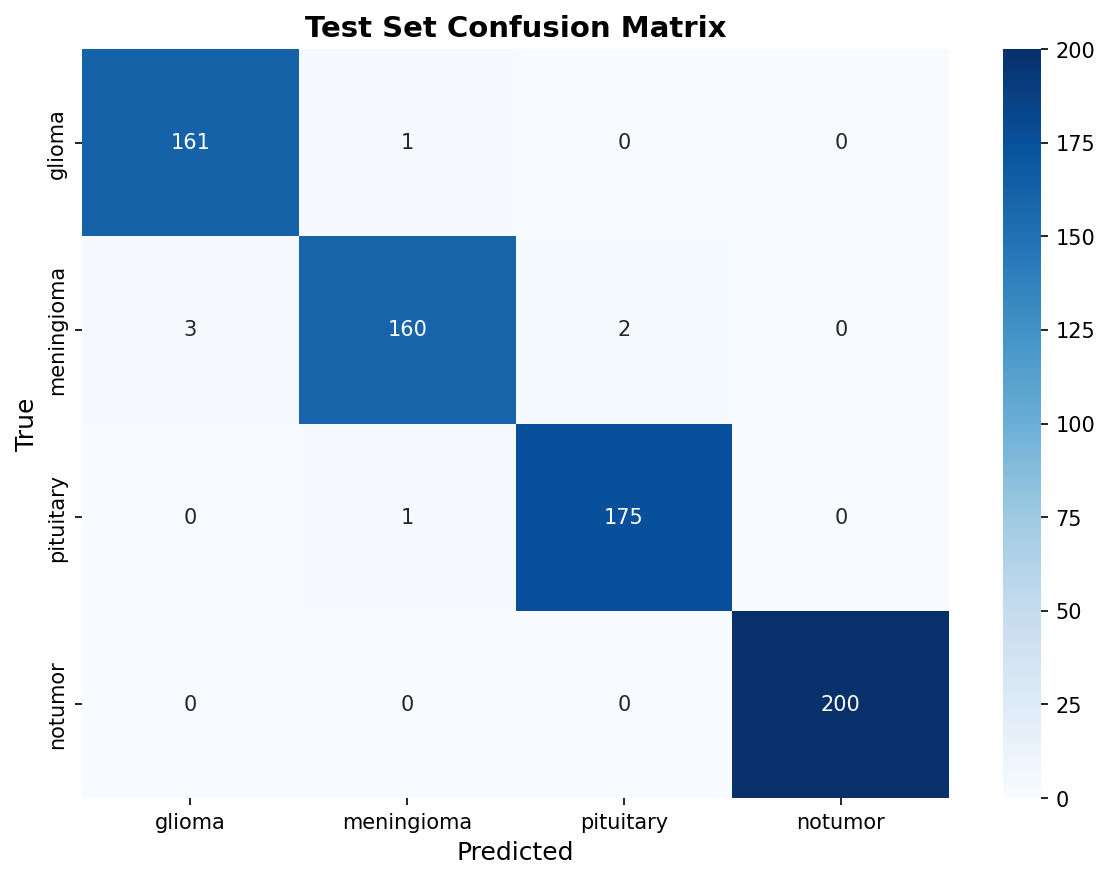
\includegraphics[width=0.5\textwidth]{figures/confusion_matrix_resunet_dual.png}
    \caption{Confusion matrix for the dual-input ResNet50 classifier.}
    \label{fig:supp_cm_resunet_dual}
\end{figure}

\begin{figure}[H]
    \centering
    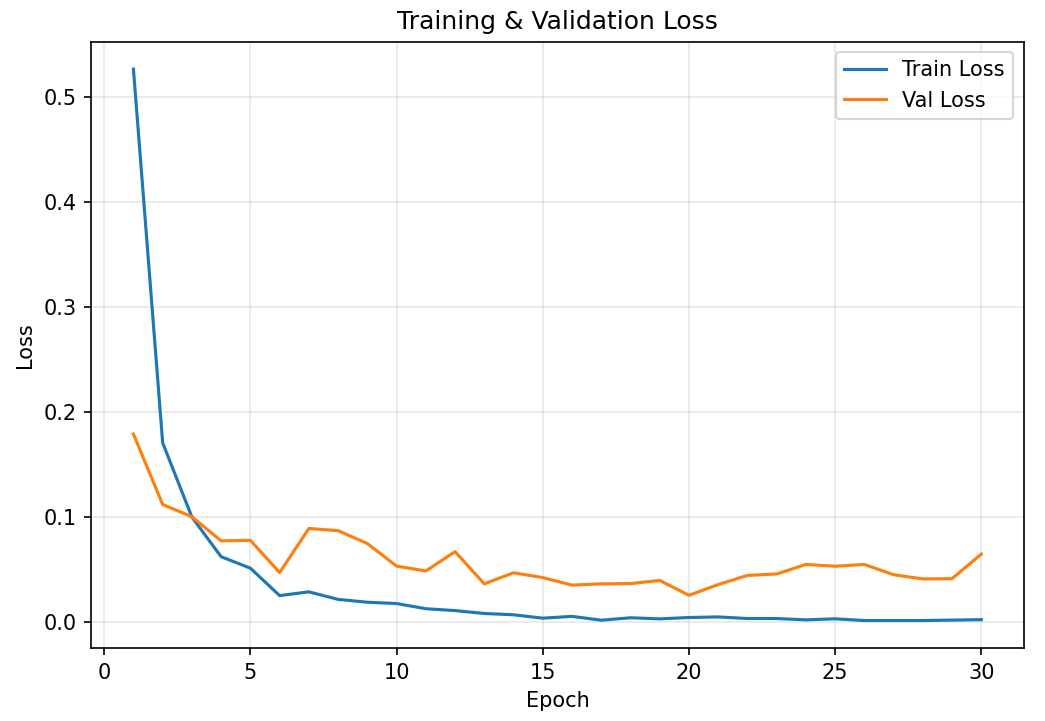
\includegraphics[width=0.7\textwidth]{figures/training_curves_resunet_dual.png}
    \caption{Training and validation curves for the dual-input ResNet50 classifier.}
    \label{fig:supp_dual_training_curves}
\end{figure}

\begin{figure}[H]
    \centering
    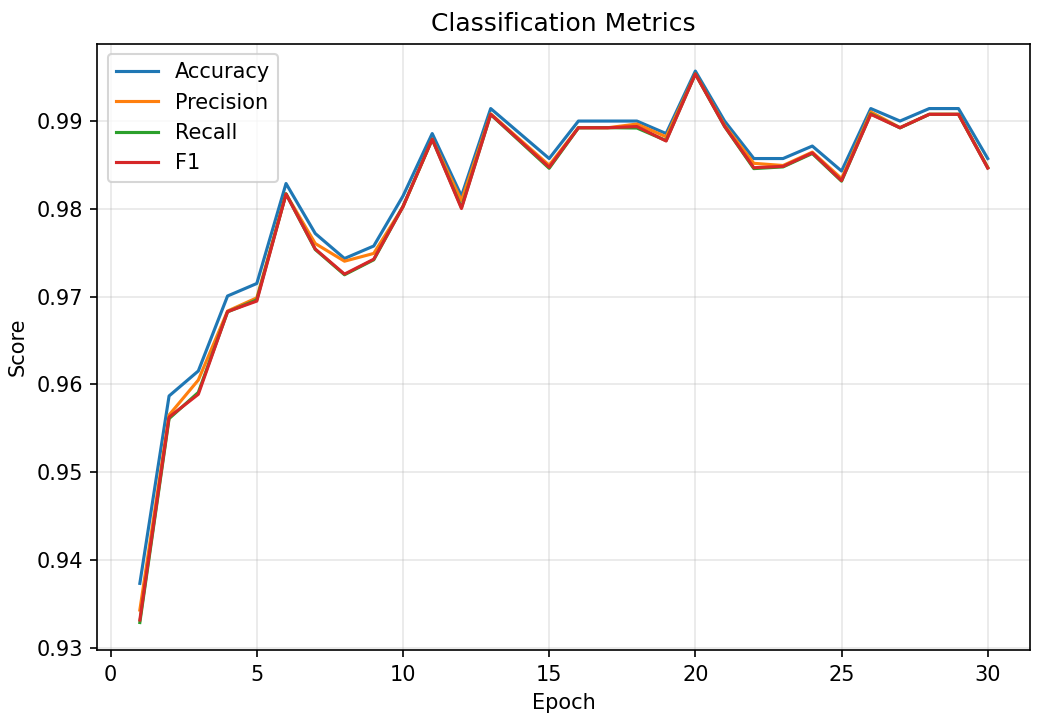
\includegraphics[width=0.7\textwidth]{figures/metric_curves_resunet_dual.png}
    \caption{Classification metric curves for the dual-input ResNet50 classifier.}
    \label{fig:supp_dual_metric_curves}
\end{figure}

\subsection*{B. Additional Qualitative Examples}
Figures~\ref{fig:supp_debug_notumor} and~\ref{fig:supp_debug_pituitary} show debugging examples from the final explainable pipeline. These examples include intermediate outputs such as the original MRI slice, available ground-truth or empty mask, predicted segmentation mask, Grad-CAM visualization, and generated VLM summary. They are useful for checking whether each stage of the pipeline behaves consistently during development.

\begin{figure}[H]
    \centering
    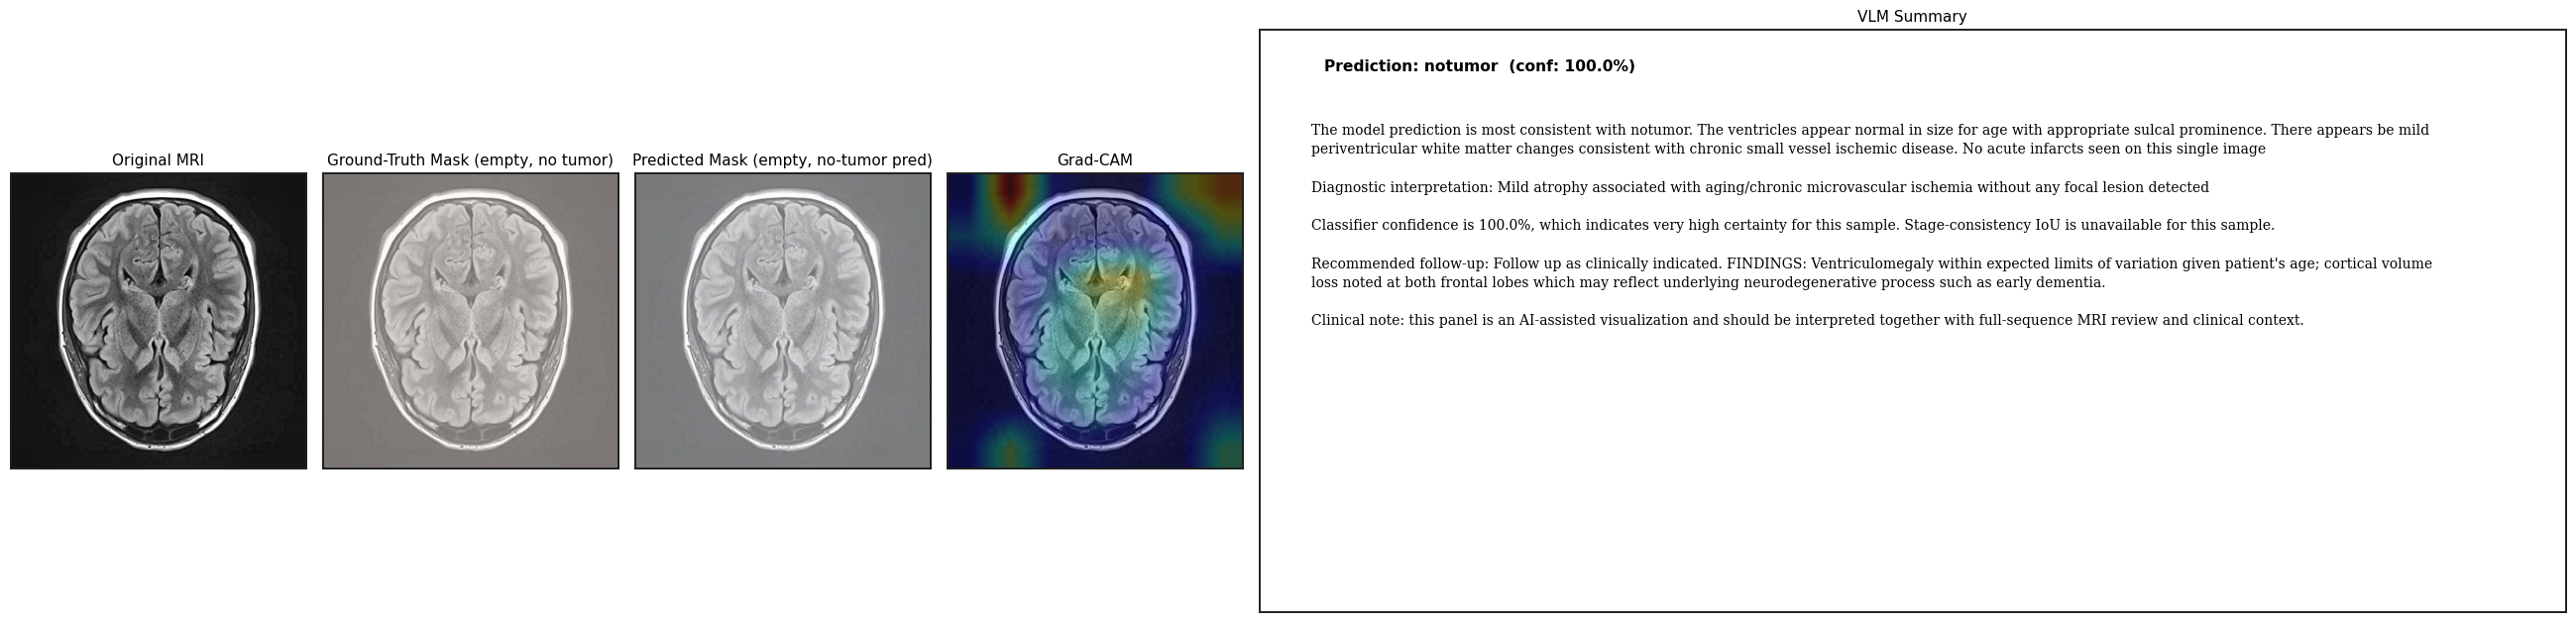
\includegraphics[width=1\textwidth]{figures/result4.png}
    \caption{Debugging example for a no-tumor case.}
    \label{fig:supp_debug_notumor}
\end{figure}

\begin{figure}[H]
    \centering
    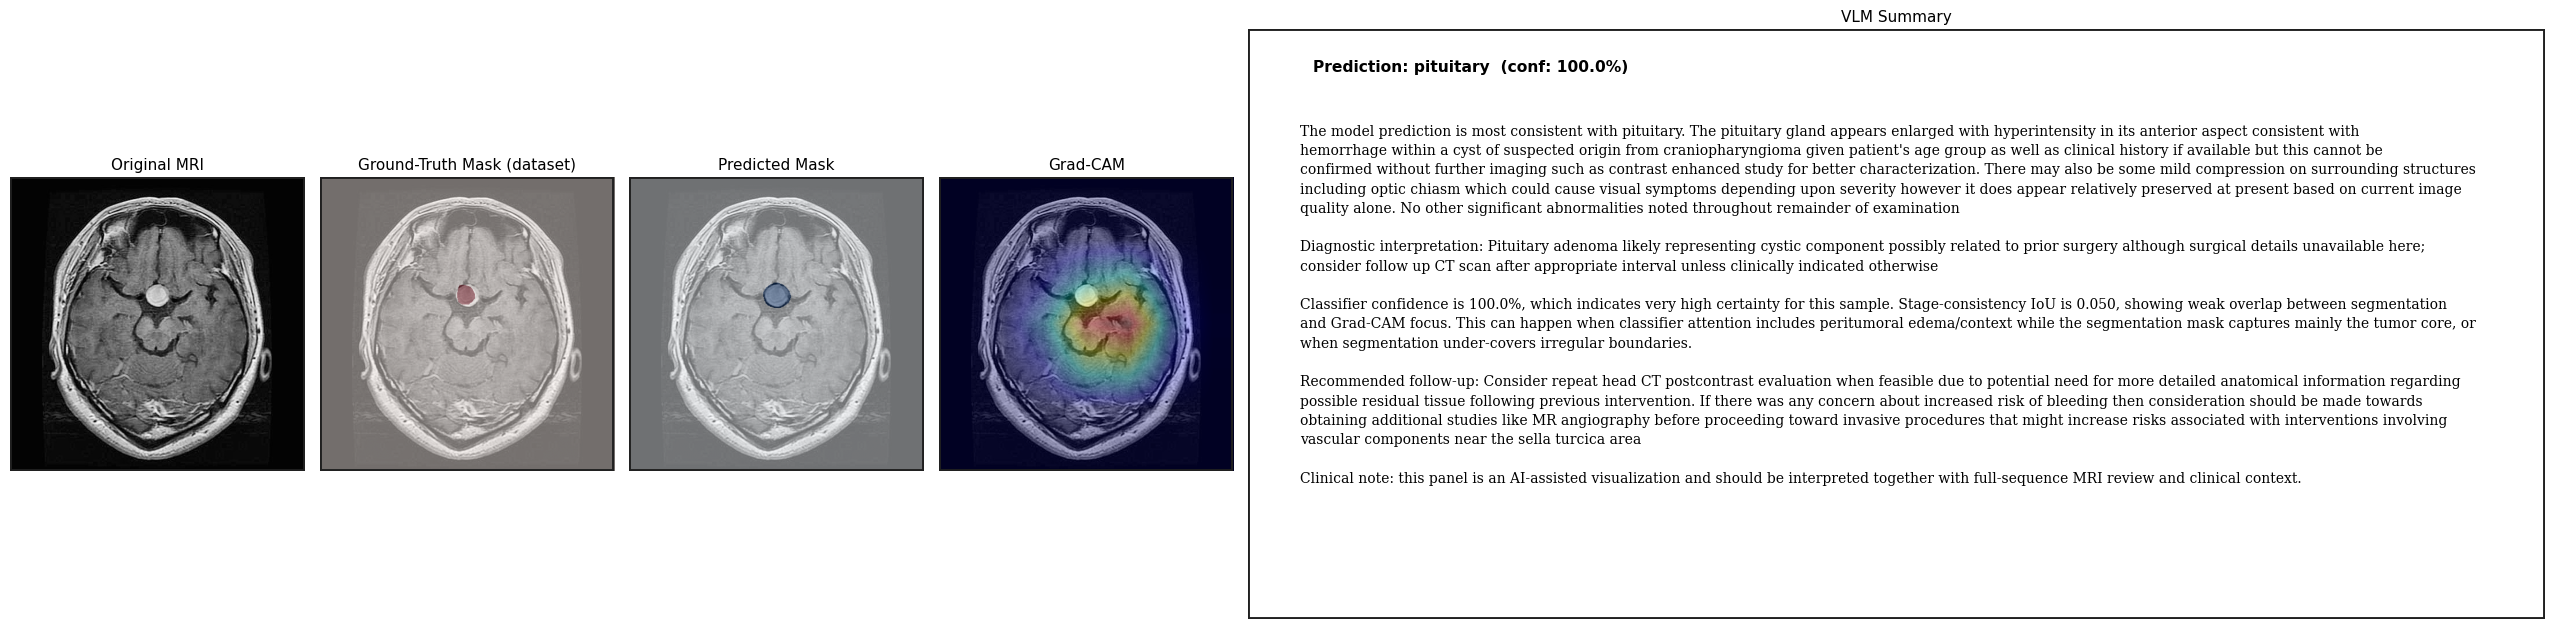
\includegraphics[width=1\textwidth]{figures/result3.png}
    \caption{Debugging example for a pituitary tumor case.}
    \label{fig:supp_debug_pituitary}
\end{figure}

Figures~\ref{fig:supp_real_notumor}, \ref{fig:supp_real_pituitary}, and~\ref{fig:supp_real_glioma} show more realistic inference examples where the ground-truth mask is not shown. These examples better reflect the expected deployment setting, where the system receives only an input MRI image and produces a predicted mask, Grad-CAM visualization, class prediction, and generated summary.

\begin{figure}[H]
    \centering
    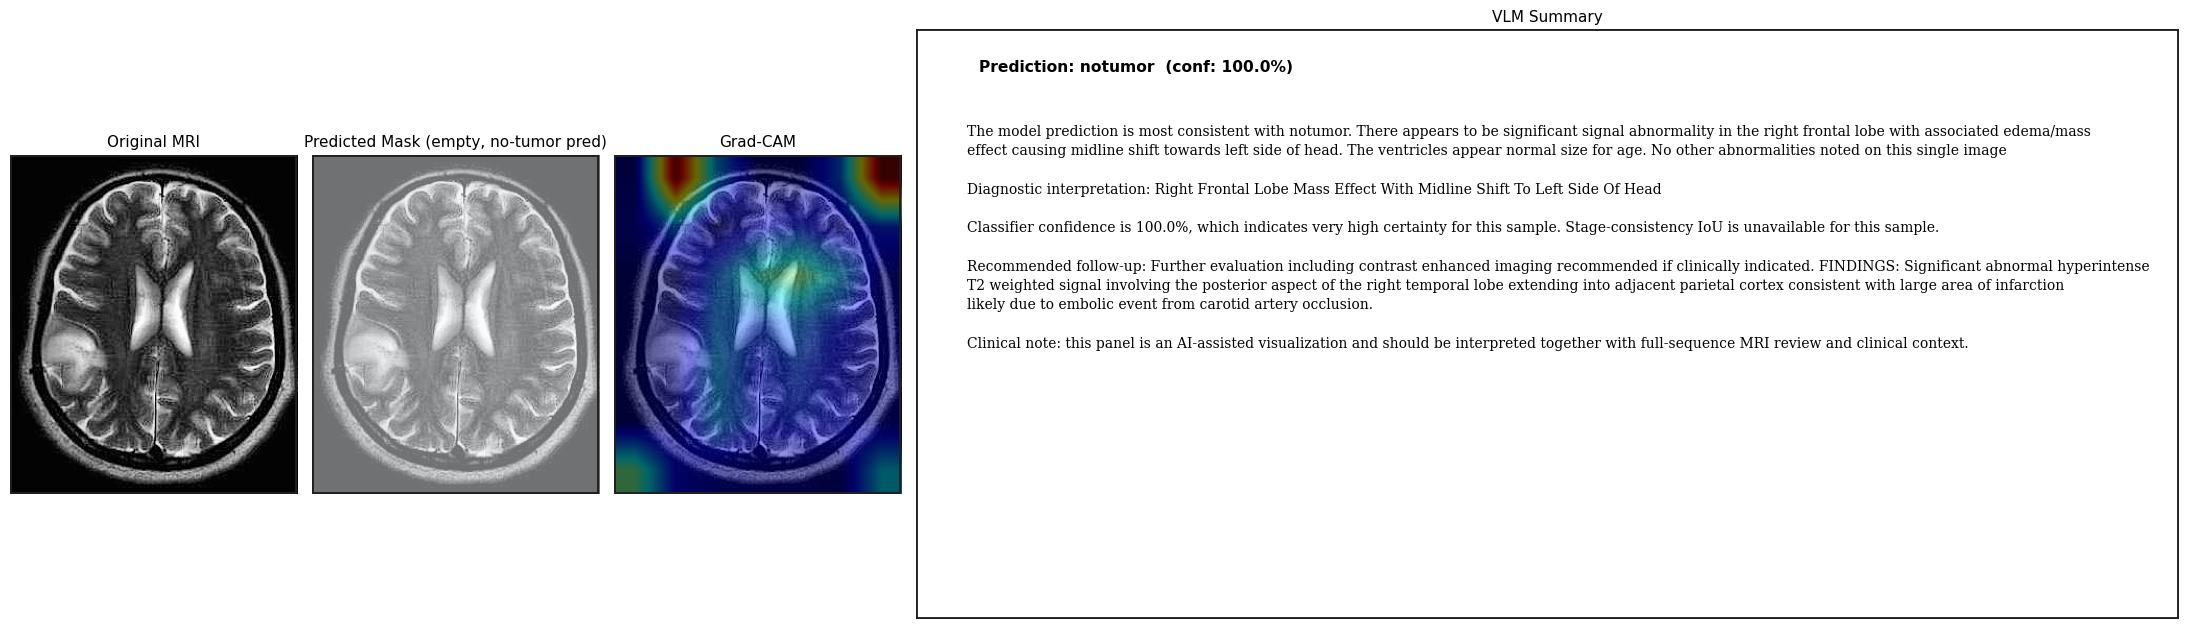
\includegraphics[width=1\textwidth]{figures/real_result2.png}
    \caption{Realistic inference example for a no-tumor case, without ground-truth mask shown.}
    \label{fig:supp_real_notumor}
\end{figure}

\begin{figure}[H]
    \centering
    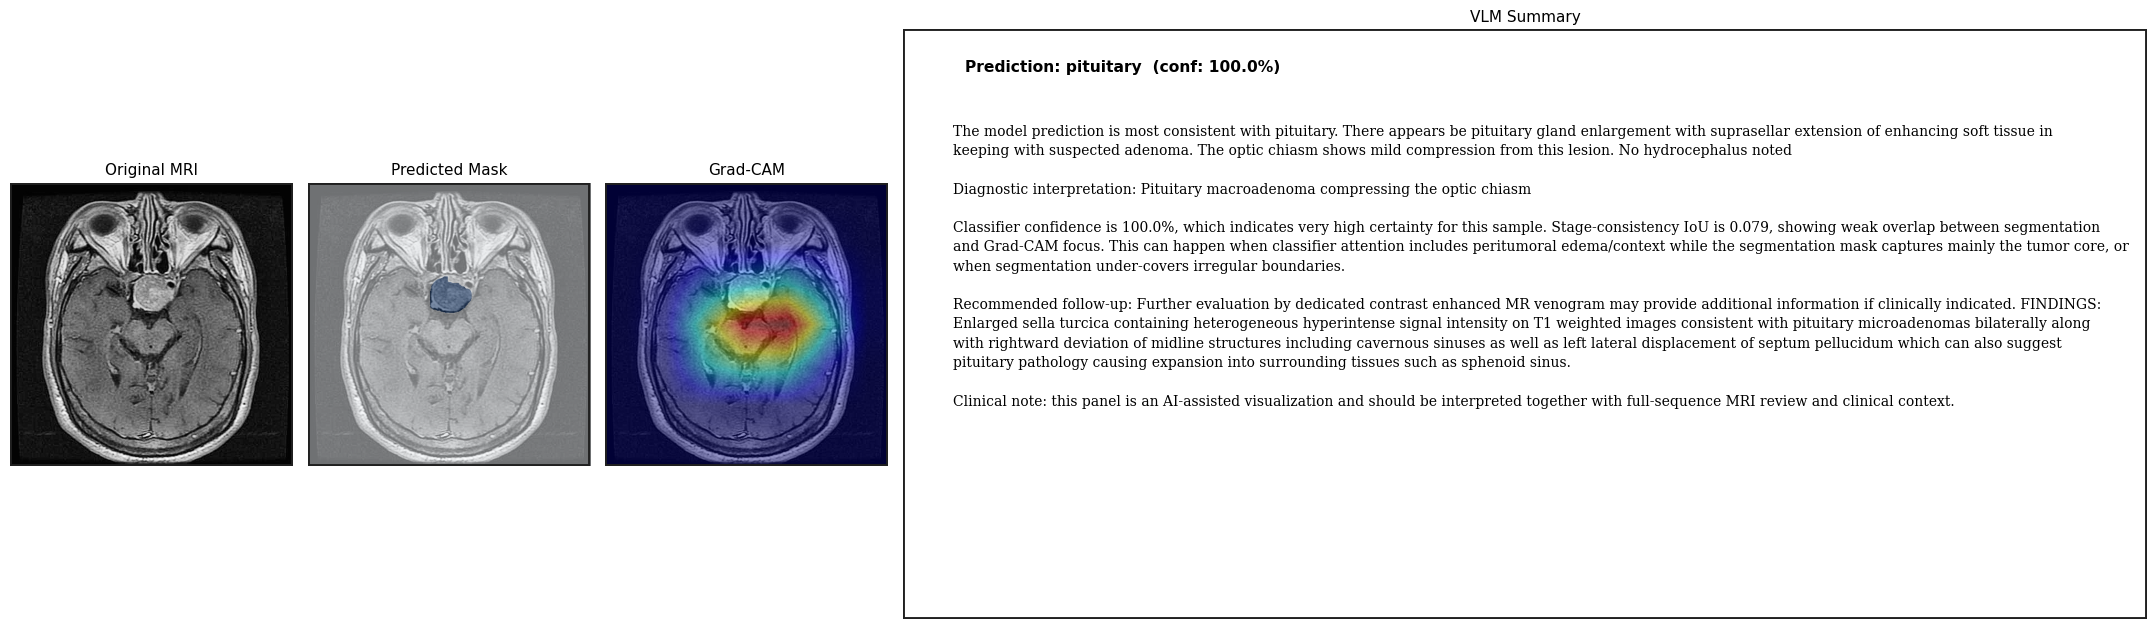
\includegraphics[width=1\textwidth]{figures/real_result1.png}
    \caption{Realistic inference example for a pituitary tumor case, without ground-truth mask shown.}
    \label{fig:supp_real_pituitary}
\end{figure}

\begin{figure}[H]
    \centering
    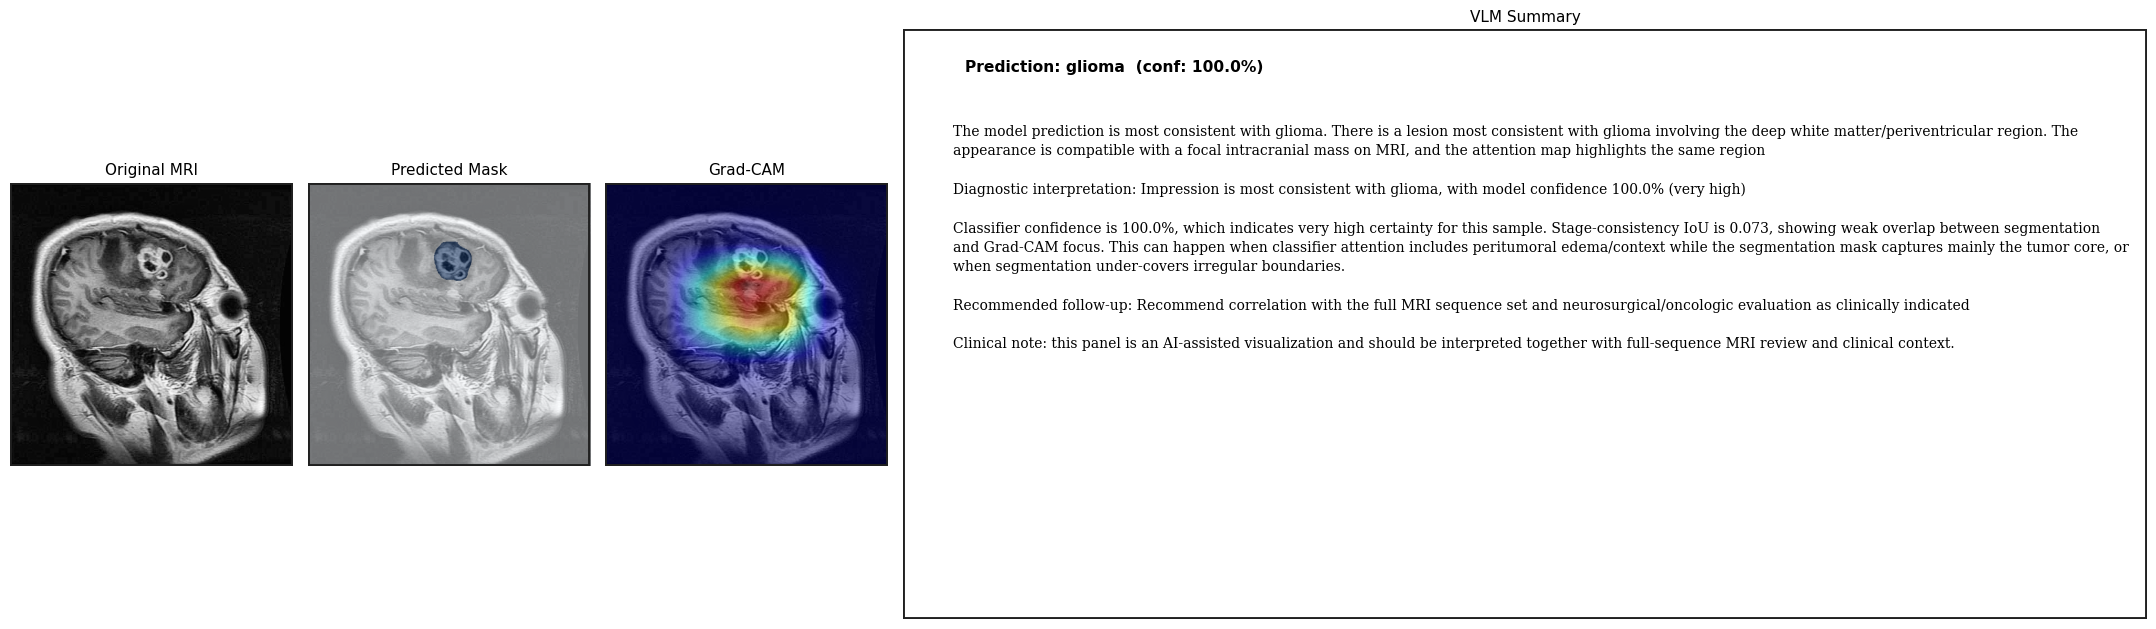
\includegraphics[width=1\textwidth]{figures/real_result3.png}
    \caption{Realistic inference example for a glioma case, without ground-truth mask shown.}
    \label{fig:supp_real_glioma}
\end{figure}

The VLM summary module is prompted in a zero-shot instruction format. The prompt conditions the model on the predicted class, confidence score, and Grad-CAM focus region, and asks it to produce a structured summary. If the generated output is malformed or inconsistent with the classifier prediction, the system falls back to a deterministic class-conditioned template. This fallback helps keep the generated explanation aligned with the model prediction.


% WARNING: do not forget to delete the supplementary pages from your submission 
% \input{sec/X_suppl}

\end{document}